\section{\SYSTEM{}: Learning Control}
\label{sec:framework}


\PUNT{To do so, we must quickly build a model of the new application
  and then control its resource usage such that it meets a desired
  performance target with minimal energy.}

\begin{figure}
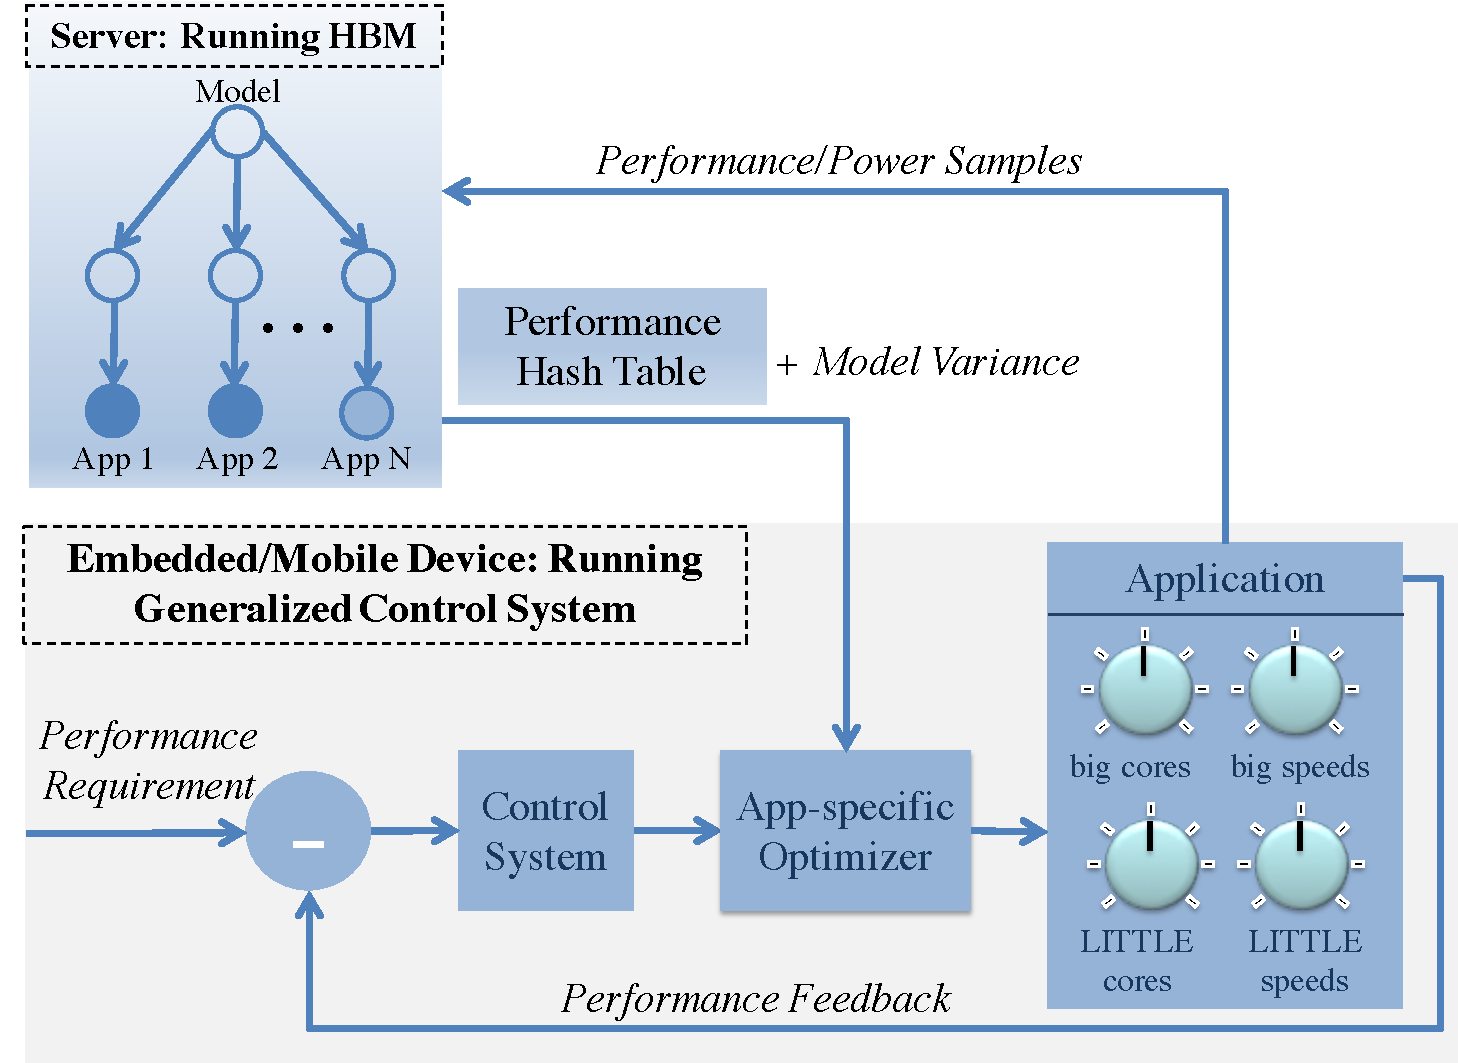
\includegraphics[width=\columnwidth]{figures/ControlLearning.pdf}
\caption{Overview of \SYSTEM{}.}
\label{fig:overview}
\end{figure}


Our goal is control theoretic resource management for streaming
applications running on embedded or mobile devices, but assuming no
assume no prior knowledge of the application.  \figref{fig:overview}
shows \SYSTEM{}'s approach to this problem.  On the local device, a
generalized control system (GCS) allocates resources to the new
application to meet its specified performance goal with minimal
energy.  The GCS starts with a generic resource model, allocates
resources according to that model, and records performance and power
for a small number of configurations.  The recorded values are sent to
a remote server which runs a hierarchical Bayesian model (HBM).  The
HBM estimates the application's performance and power in all other
configurations and extracts those that are Pareto-optimal in the
performance/ power tradeoff space.  These configurations are packaged
in a special data structure -- the performance hash table (PHT) -- and
sent to the GCS.  Using the PHT, the GCS selects an energy minimal
resource configuration in constant time ($O(1)$).  The server also
sends back the model's variance, which the GCS uses to customize
control to the model's uncertainty. By communicating variance,
\SYSTEM{} guarantees convergence to the performance goal even though
it starts with no prior knowledge of the streaming application.

\PUNT{
The remainder of this section details \SYSTEM{}.  We begin by
describing a typical control design for a computer system and
illustrate how it fails to generalize.  We then describe \SYSTEM{}'s
generalized control system.  Next we discuss how \SYSTEM{} turns the
generalized control signal into specific resource configurations using
a model.  We then describe how to use a hierarchical Bayesian model to
estimate resource performance and power tradeoffs.  We then describe
the performance hash table that encodes the learned model. We conclude
with some brief analysis of the approach, with detailed analysis
provided in an appendix.
}

\subsection{Traditional Control for Computing}
\PUNT{
A controller has a performance goal (corresponding to a
quality-of-service or real-time constraint) and adjusts system resource
usage to see that the goal is met. Following is the general formulation for a controller, where the response is assumed to be linearly related to the effect.
\begin{equation}
  effect(t) = \alpha \cdot response(t-1) + \delta \label{eqn:clock}
\end{equation}
A control system might adjust processor frequency to ensure that a performance
goal is met \cite{lefurgy2008power}.  Even better, an optimal controller would
use the minimal clockspeed to meet the performance requirement.


To turn clockspeed into performance a controller needs a model
relating these two values.  A physical model, directly mapping clockspeed to performance
is difficult -- a hypothetical model might account for instruction
mixes, memory hierarchy, memory latency, synchronization overheads,
etc.  Building such a model is tedious and error-prone process and
that is before we address system dynamics (\eg applications
transitioning from memory to compute bound).  Instead, control systems
use relatively simple difference models\footnote{Continuous time
  systems would use differential equations, but as time in computers
  is inherently discretized we restrict ourselves to discussion of
  difference equations which are appropriate for discrete time
  systems.}.
}

%example difference model -- built into the controller

\PUNT{

Continuing the example of controlling performance with clockspeed, a
simple model appropriate for control would be to assume that the
performance is a linear function of the clockspeed:
\begin{equation}
  perf(t) = \alpha \cdot clockspeed(t-1) + \delta \label{eqn:clock}
\end{equation}
Here, the observed performance $perf(t)$ is predicted as some constant
$\alpha$ times the clockspeed applied at the previous time step,
$clockspeed(t-1)$, plus some noise, $\delta$ drawn from a Gaussian
distribution.  This simple linear difference model ignores low-level
details like instruction mix, and instead uses feedback, predicting
behavior of the next time step as a function of the previous time
step.  Using the relationship of \eqnref{clock}, we can synthesize a
simple controller that is provably convergent to the desired
performance:
\begin{eqnarray}
  error(t) &=& goal - perf(t) \label{eqn:clock-error} \\
  clockspeed(t) &=& clockspeed(t-1) - \frac{error(t)}{\alpha}
  \label{eqn:clock-control}
\end{eqnarray}
}


Using traditional control design, we can turn LAVAMD's model -- from
\figref{fig:lavamd_model} -- into a controller.  The model follows
directly from the linear fit:
\begin{equation}
  perf(t) = 2.95 \times 10^{-6} \cdot clock(t-1) + \delta \label{eqn:clock}
\end{equation}
This model states the observed $perf(t)$ is the slope of our model
times the clockspeed applied at the previous time step, $clock(t-1)$,
plus some Gaussian noise $\delta$.  This simple linear difference
model ignores low-level details like instruction mix, and instead uses
feedback, predicting behavior of the next time step as a function of
the previous time step.  Using \eqnref{clock}, we synthesize a simple
controller that is provably convergent to the $goal$ performance
\cite{ICSE2014}:
\begin{eqnarray}
  error(t) &=& goal - perf(t) \label{eqn:clock-error} \\
  clock(t) &=& clock(t-1) - \frac{error(t)}{ 2.95 \times 10^{-6}}
  \label{eqn:clock-control}
\end{eqnarray}



% Can we make the model a tunable parameter?
The controller design in \eqnref{clock-control} provides formal
guarantees that it will converge to the desired performance ($goal$ in
\eqnref{clock-error}) and it bounds convergence time.  These
guarantees, however, are predicated on the model's accuracy; \ie{} how
well the slope in \figref{fig:lavamd_model} approximates measured
performance.  This value is highly dependent on the particular
application under control.  This model will not work for applications
that are memory-bound and do not speed up with increasing clockspeed.
As we add more resources to the controller we turn the scalar
equations of this example into matrix equations
\cite{METE,josep-isca2016}.  Whether scalar or matrix, the equations
and the formal guarantees they embody are reliant on accurate models
of resource interaction.  Since we cannot build one model for all
applications, we want to tune the control models to individual
applications.

\subsection{Generalized Control System}
In the above example, the controller is application-specific because
it directly incorporates the slope of the model into the control
equations.  Our goal is to build a controller where those key
parameters can be tuned online.  To do so, we use the classic computer
science trick of adding a layer of indirection as illustrated in
\figref{fig:overview}.  Instead of directly controlling resources
using an application-dependent model, we will control \emph{speedup}
and pass that speedup value to a separate module that turns desired
speedup into an energy-minimal resource configuration using the
learned models.  We first describe our formulation for controlling
speedup and then converting that speedup into resource allocations.

\subsubsection{Controlling Speedup}
Analogous to \eqnref{clock} we write a simple difference model
relating speedup to performance:
\begin{equation}
  perf(t) = b \cdot speedup(t-1) + \delta \label{eqn:speedup}
\end{equation}
where $b$ is the application's \emph{base speed}: defined as the speed
when all resources are available.  While $b$ is application specific,
it is easy to measure online, by simply allocating all resources. Such
a configuration should not violate any performance constraints
(although it is unlikely to be energy efficient) so it is safe to take
this measurement without risk of violating performance constraints.

With this model, the control law is simply:
\begin{eqnarray}
  error(t) &=& goal - perf(t) \label{eqn:speedup-error} \\
  speedup(t) &=& speedup(t-1) - \frac{error(t)}{b}
  \label{eqn:speedup-control}
\end{eqnarray}
which states that the speedup at time $t$ is a function of the
previous speedup, the error at time $t$ and the base speed.  This is a
very simple \emph{deadbeat} controller that provides all the standard
control theoretic formal guarantees.


By measuring base speed online while the application runs, we tune the
control to a specific application; using this definition of base
speed, most speedups will be less than one.  We can further generalize
\eqref{eqn:speedup-control} as:
\begin{equation}
speedup(t) = speedup(t-1) - \frac{1 - \rho(t)}{b}.error(t)
\end{equation}
where $0 \le \rho(t) < 1$ is a pole of the controller's characteristic
equation.  At small values of $\rho(t)$ the controller will work to
eliminate error very quickly, but it may overreact to noise or
inaccuracies in the model.  Larger values of $\rho(t)$ make the system more
robust at the cost of reduced convergence time.  \emph{Dynamically
  setting the pole to the HBM's output will be a key of combining
  control and learning.} First, however, we address the challenging
problem of converting an abstract speedup into an actual resource
allocation.


\subsubsection{Converting Speedup to Resource Allocation}
We need to map \eqnref{speedup-control}'s speedup into a resource
allocation.  On our example ARM big.LITTLE architecture that
specifically means mapping speedup into an allocation of big and small
as well as a speed for both (on our system clocks big and little cores
separately).

The primary challenge is that the HBM produces a discrete non-linear
function of resource usage into speedup and powerup, while
\eqnref{speedup-control} is a continuous linear function.  We bridge
this divide by assigning time to resource allocations such that the
average speedup over a control interval is that produced by
\eqnref{speedup-control}.

We call an assignment of time to resources a schedule. There are
typically many schedules that meet a particular performance
requirement and we want to find a minimal energy schedule. Given a
time interval $T$, a speedup requirement $speedup(t)$ to average over
the time interval, and a configuration set of size $C$ , we formalize
this problem as:
\begin{eqnarray}
  \minimize_{\mathbf{\tau} \in \R^{C}} && \sum_{c=0}^{C-1} \tau_c \cdot p_c \label{eqn:power}  \\
  \st %&& \nonumber\\
  && \sum_{c=0}^{C-1} \tau_c \cdot s_c =  speedup(t)T \label{eqn:work} \\
  && \sum_{c=0}^{C-1} \tau_c =  T \label{eqn:deadline} \\
  && 0 \le \tau_c \le T, \qquad \forall c \in \{0,\ldots,C-1\} \label{eqn:time}
\end{eqnarray}
where $p_c$ and $s_c$ are configuration $c$'s estimated powerup and
speedup; $\tau_c$ is the time to spend in configuration $c$.
\eqnref{power} simply states that the objective is to minimize energy
(power times time).  \eqnref{work} states that the average speedup
must be maintained, while \eqnref{deadline} requires the time to be
fully utilized.  \eqnref{time} simply avoids negative time.


\subsection[Learning Power/Performance Tradeoffs]{Hierarchical Bayesian Models}
\PUNT{
\begin{figure}
\centering
  \subfloat[]
  {
    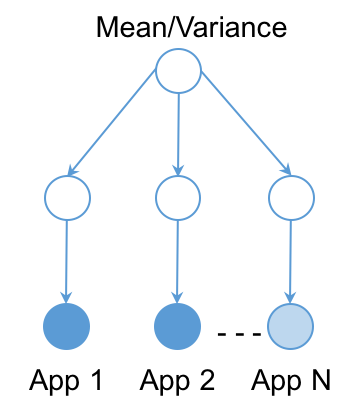
\includegraphics[width=.2\textwidth]{figures/HBM.png}
  }
  \caption{ A Hierarchical Bayesian model.  The arrows represent
    dependences, circles are random variables, white circles are
    hidden variables that cannot be observed and must be learned,
    solid circles represent fully observed data, and shaded circles
    represent partially observed data.}
\label{fig:learning-models}
\end{figure}

\begin{figure*}

  \subfloat[]
  {
    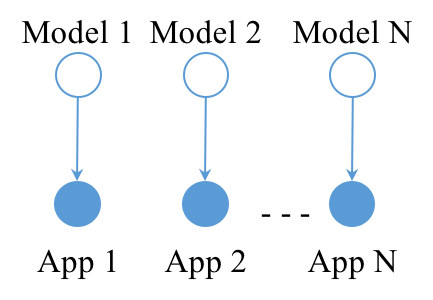
\includegraphics[width=.33\textwidth]{figures/Online.png}
    \label{fig:online}
  }
  \subfloat[]
  {
    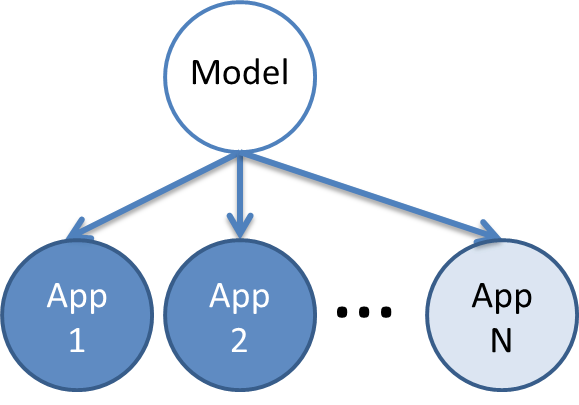
\includegraphics[width=.33\textwidth]{figures/Offline.png}
    \label{fig:offline}
  }
  \subfloat[]
  {
    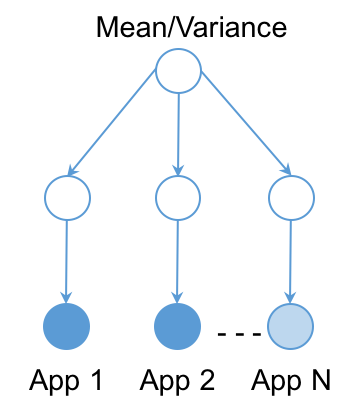
\includegraphics[width=.33\textwidth]{figures/HBM.png}
    \label{fig:HBM}
  }
  \caption{ Comparison of online (a) offline (b) and hierarchical
    Bayesian models (c).  The arrows represent dependences, circles
    are random variables, white circles are hidden variables that
    cannot be observed and must be learned, solid circles represent
    fully observed data, and shaded circles represent partially
    observed data.  The online model is concerned only with the
    current application (labeled N), the offline model combines all
    observations into one model, and the HBM builds per-application
    models, but makes them conditionally dependent on one another so
    that prior observations can be used to increase the accuracy of
    the model built for application N.}
\label{fig:learning-models}
\end{figure*}
}

Assuming no prior knowledge of the application, we estimate its power
($p_c$) and performance ($r_c$) in configuration $c$.
\PUNT{Specifically, we take observations of performance and power in a
  resource configuration and predict (1) how future applications will
  perform or (2) how different resource allocations affect the current
  application.}  \SYSTEM{} uses a hierarchical Bayesian model (HBM) to
turn observations of an application's performance and power into
predictions about how other, unobserved resource allocations will
affect performance and power.  The HBM provides a statistically sound
framework for learning across applications and devices; \ie{} it
handles the non-convex tradeoff spaces heterogeneity produces (\eg{}
\figref{fig:lavamd_contour}).

The HBM provides balance between completely online approaches -- which
consider only the current application -- and offline approaches --
which consider only prior applications approaches.  \PUNT{ Each
  application has its own model, allowing specificity, but these
  models are conditionally dependent on some underlying probability
  distribution with a hidden mean and co-variance matrix.  In
  practice, the HBM will estimate a model for a new application using
  a small number of observations and combining those observations with
  the large number of observations previously made of similar
  applications.  Rather than over-generalizing, the HBM will use only
  similar applications to learn models.  In addition, the HBM's
  accuracy increases as more applications are observed because more
  different types of behavior are represented in the pool of prior
  knowledge.  Of course, the computational complexity of learning also
  increases with increasing applications, but this is why we offload
  the learning to a remote server.  } Consider a simplified example.
Suppose we have observed many prior applications, all of which are
either completely compute-bound or completely memory-bound, and we
have an equal number of both.  The only resource we can allocate is
clockspeed, which will increase the performance of compute-bound
applications, but not memory-bound ones.  When we need to work with a
new application, we need to estimate its response to clockspeed.  The
online model does not use prior knowledge, but will observe many
different clock speeds for the new application, leading to high
overhead.  A fully offline model predicts the mean response of prior
applications, meaning it will over-allocate speed to memory-bound
applications and under-allocate to compute-bound ones.  The HBM takes
a small number of observations and combines those with prior
knowledge: if the new observations show that clockspeed has no effect
on performance the HBM will use only the prior memory bound
applications to build its model, otherwise, it will use the
compute-bound applications.  In practice, the HBM can learn much more
complicated tradeoffs by combining observations of the new application
with prior knowledge of different types of behavior.

\PUNT{
When selecting a learning framework we must find a tradeoff between
the specific and the general; \ie{} between frameworks that build
application-specific models and frameworks that combine observations
across applications.  For example, the key to energy efficiency on
heterogeneous mobile systems is knowing when to make use of the
smaller, low-power cores \cite{}.  An application-specific model will
capture that precisely, but may require many observations before
producing the correct model.  A more general model will capture the
trend, \eg when most applications should transition, but this general
model might miss the key inflection point for some applications.  We
refer to application-specific models as \emph{online} because they
build models for the current application and do not incorporate
knowledge of other applications.  We refer to general models as
\emph{offline} as they use prior observations of other applications to
predict the behavior of a new application.
}

Suppose our system has $n = |\mathcal{C}|$ configurations.  \PUNT{We
  have a \textit{target application} whose energy we wish to minimize,
  while meeting a performance requirement (as in
  \eqref{eq:controller}).}  Additionally, we have a set of $m-1$
applications whose performance and power are known (\ie{} they have
been measured offline). Let the vector $\y_i \in \R^{n}$ represent
application $i$'s power or (performance) estimate in all $n$
configurations; \ie{} the $c$th component of $\y_i$ is the power for
application $i$ in configuration $c$ (or $\y_i[c] = p_c$).  Also, let
$\{\y_i\}_{i =1}^m$ be shorthand for the power estimates of all
applications.  Without loss of generality, we assume the first $m-1$
columns, \ie{} $\{\y_i\}_{i =1}^{m-1}$ represent the data for those
applications whose power consumption is collected offline.  The $m$th
column, $\y_m$ represents the power consumption for the new, unknown
application.  We have a few observations for this application.
Specifically, for the $m$th application we have observed
configurations belonging to the set $\Omega_m$ where $|\Omega_m| \ll
n$.  The HBM estimates application $m$'s power for all unobserved
configurations using the following statistical model:
\begin{equation}
\begin{aligned}
\y_i \vert \z_i  &\sim N( \z_i, \sigma^2 \I),\\
\z_i \vert \mu,\Sigma &\sim N(\mu, \Sigma),\\
\mu, \Sigma &\sim N(\mu_0,\Sigma / \pi)IW(\Sigma | \nu, \Psi),
\end{aligned}
\label{eq:HBN}
\end{equation}

where $\y_i \in \R^n, \; \z_i \in \R^n, \; \mu \in \R^{n}, \; \Sigma
\in \R^{n\times n}$. In this model the power (denoted by $\y_i$) of
the $i^{th}$ application, is drawn from multivariate-Gaussian
distribution with mean $\z_i$ and a diagonal covariance matrix
$\sigma^2\I$.  Similarly, $\z_i$ is from multi\-variate-Gaussian
distribution with mean $\mu$ and covariance $\Sigma$. And, $\mu$ and
$\Sigma$ are jointly drawn from normal-inverse-Wishart distribution
with parameters $\mu_0, \pi,\Psi, \nu$.  Our model's parameters are
$\mu,\Sigma$, whereas, $\mu_0, \pi,\Psi, \nu$ are the
hyper-para\-meters, which we set as $\mu_0 = 0, \pi = 1,\Psi = \I, \nu =
1$.  We solve the above equations using an
\emph{estimation-maximization} algorithm to get a value of $z_M$,
which serves as an estimator for the target application.




\subsection{Encoding Learned Models}
Given the HBM's estimates of speedup and power, we know need to solve
\eqnrref{power}{time}.  The GCS solves this on the local device, so
solution must be found efficiently.  To achieve this efficiency we (1)
exploit the structure of this particular optimization and (2) encode
the HBM's model in a performance hash table (PHT).  Combining these
two ideas we solve \eqnrref{power}{time} in constant ($O(1)$) time.

Kim et al. analyze heuristic solutions to the problem of minimizing
energy while meeting a performance constraint \cite{kim-cpsna}.  They
observe that there must be an optimal solution with the following
properties:
\begin{itemize}
\item At most two of $\tau_c$ are non-zero, meaning that at most two
  configurations will be used in any time interval.
\item If you chart the configurations in the power and performance
  tradeoff space the two configurations with non-zero $\tau_c$ lie on
  the lower convex hull of the power performance tradeoff space.
\end{itemize}
We use these two facts to construct a constant time algorithm for
finding the optimal solution online.

\begin{figure}
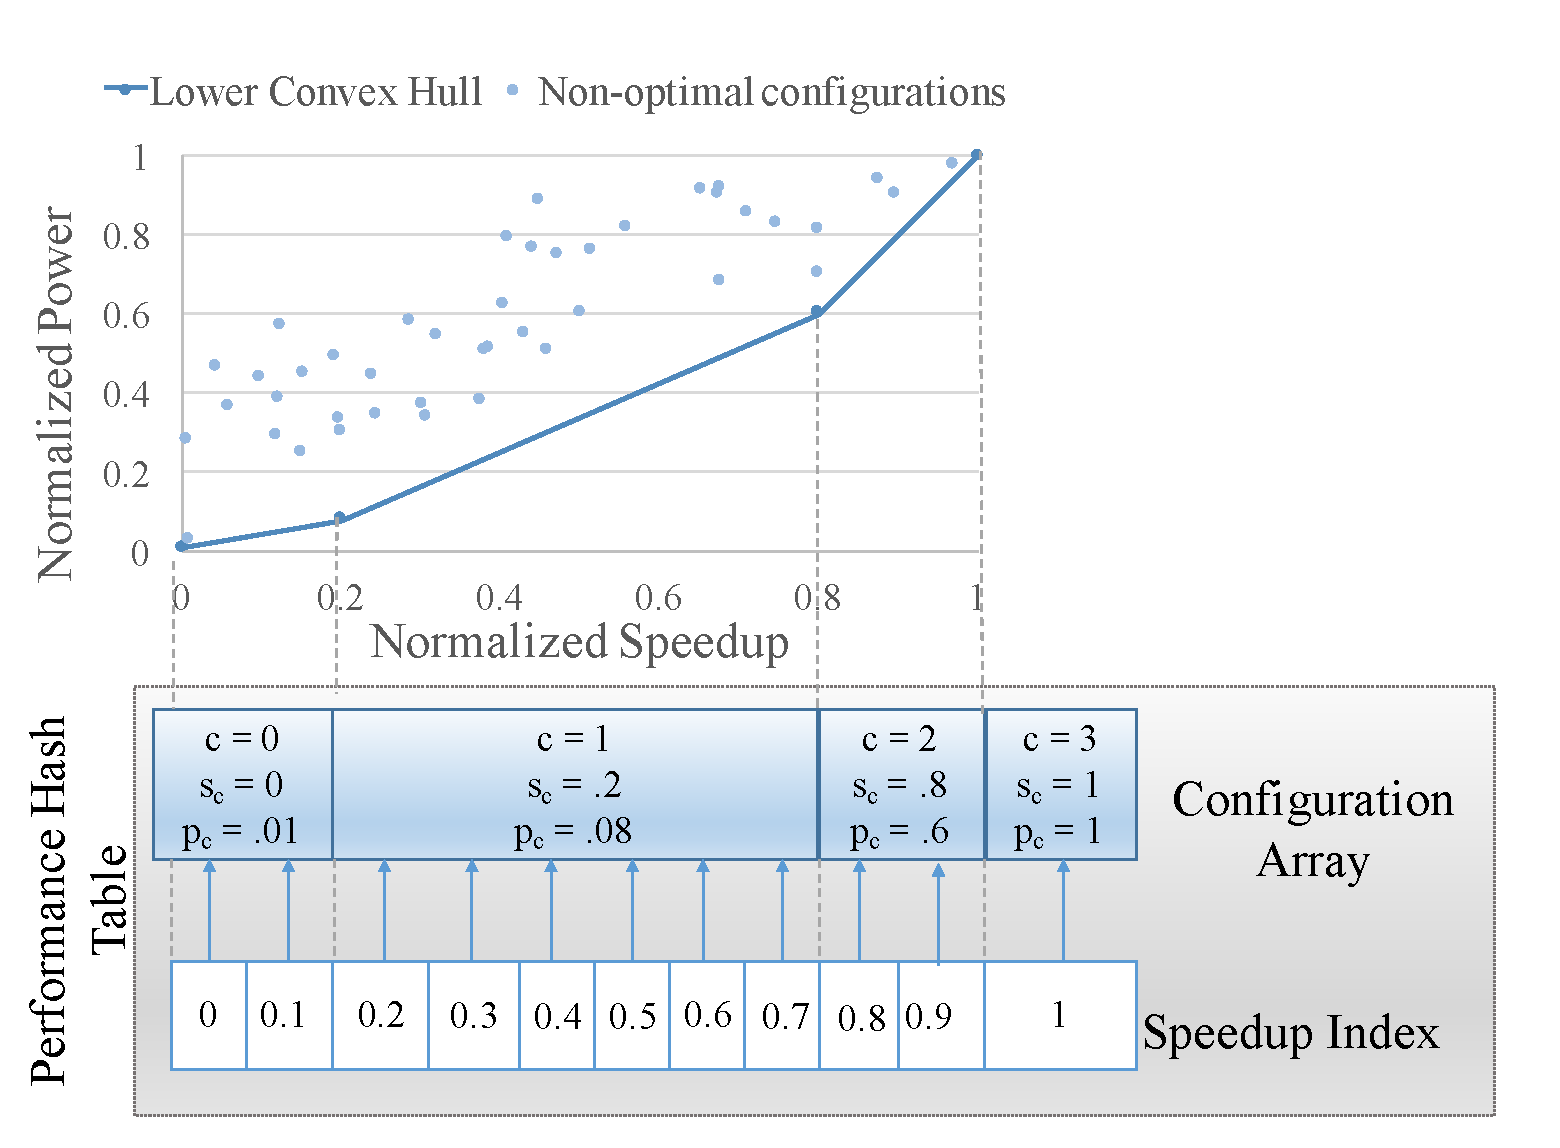
\includegraphics[width=\columnwidth]{figures/performance-hash-table.pdf}
\caption{Data structure to efficiently convert required speedup into a
  configuration.}
  \label{fig:pht}
\end{figure}

The PHT (illustrated in \figref{fig:pht}) only contains points on the
lower convex hull of the power/performance tradeoff space.  It
consists of two arrays: an array of pointers that point into a second
array, which stores the configurations on the convex hull sorted by
speedup.  Recall that speedups are computed relative to the base speed
which uses all resources.  We therefore know the largest speedup is 1,
so we need only concern ourselves with speedups less than 1.  The
first table, of pointers has a \emph{resolution} indicating how many
decimal points of precision it captures.  The example in
\figref{fig:pht} has a resolution of $0.1$.  Each pointer in the first
table points to the configuration in the second array that has the
largest speedup less than or equal to the index.

To use the table, the optimizer (\figref{fig:overview}) receives a
speedup $speedup(t)$ from the controller.  It converts this into two
configurations referred to as $hi$ and $lo$.  To find the $hi$
configuration, the translator clamps the desired speedup to the
largest index lower than $speedup(t)$ and then walks forward until it
finds the first configuration with a speedup higher than $speedup(t)$.
This configuration is $hi$.  To find the $lo$ configuration, the
translator clamps the desired speedup to the smallest index higher
than $speedup(t)$ and then walks backwards until it finds the
configuration with the largest speedup less than $speedup(t)$.

For example, consider the PHT in \figref{fig:pht} and an optimizer
meeting $speedup(t) = .65$.  To find $hi$, the optimizer indexes at .6
and walks up to find $c=2$ with $s_c=.8$, setting $hi = 2$.  To find
$lo$, the optimizer indexes the table at .7 and walks backward to find
$c=1$ with $s_c=.2$, setting $lo = 1$.

Finally, the optimizer sets $\tau_{hi}$ and $\tau_{lo}$ by solving the
following set of equations:
\begin{eqnarray}
  T &=& \tau_{hi} + \tau_{lo}    \label{eqn:s1} \\
  speedup(t) &=& \frac{s_{hi} \cdot \tau_{hi} + s_{lo} \cdot \tau_{lo}}{T} \label{eqn:s2}
\end{eqnarray}
In these equations, $speedup(t)$ is the speedup requested by the
controller and $s_c$ are speedups estimated by the learner.  By
solving \eqnsref{s1}{s2}, the optimizer has turned the controller's
speedup into a schedule of resource allocations using the models
provided by the HBM.

\PUNT{ Provided that the resolution is large enough to get a good
  spread of configurations to indices, the translator will always
  index the configuration array at most one entry from where it needs
  to be.  Thus, the entire translation process runs in constant time
  -- assuming that the learner is responsible for building the PHT
  once before passing it on to the translator.  This efficiency comes
  at a cost of memory usage -- many of the entries in the speedup
  index table will point to redundant locations in the configuration
  array.  We think that this is a reasonable tradeoff to make in
  practice as the code that runs on the mobile device must be fast or
  we risk wasting energy while trying to save energy.  In practice, we
  recommend a table of size 100 which provides a sufficient resolution
  and is not too wasteful of space.}


\subsection{Analysis}
%\subsubsection{Algorithmic Analysis}

\noindent \textbf{Control System Complexity} The GCS (see Algorithm
\ref{alg:gcs}) runs on the mobile or embedded device; each controller
invocation is $O(1)$ .  The only part that is not obviously constant
time is the PHT lookups.  Provided the PHT resolution is sufficiently
high to avoid collisions, then each PHT lookup requires constant time.
\begin{algorithm}[t]
\caption{Generalized control system}
\label{alg:gcs}
\begin{algorithmic}
\REQUIRE Initialize the controller with random configurations. Send power and performance samples to server and get performance hash table(PHT) from the server.
\WHILE{$True$}
    \STATE    Measure streaming application performance 
    \STATE    Compute required speedup (Equation \eqref{eqn:speedup})
    \STATE    Lookup $s_{hi}$ and $s_{lo}$ with PHT
    \STATE    Compute $\tau_{hi}$ and $\tau_{lo}$ (Equations \ref{eqn:s1} \& \ref{eqn:s2})
    \STATE    Configure to system to $hi$ $\&$ sleep $\tau_hi$.
    \STATE    Configure to $lo$ $\&$ sleep $\tau_lo$.
\ENDWHILE
\end{algorithmic}
\end{algorithm}


\noindent \textbf{Learning System Complexity} We run our learning
system on a remote server because the Hierarchical Bayesian Model
(HBM) is a relatively complex algorithm and it utilizes data from
other applications which can be stored in advance on the server
machines, allowing consolidation of data across similar devices.  The
time complexity for the HBM is $O(mn^3)$ where $m$ is the number of
applications and $n$ is the number of configurations.  Second step,
creating convex hull for the PHT takes $O(n log(n))$.

\subsection{Control Theoretic Formal Guarantees}
\label{sec:guarantees}
As mention above, the pole $\rho(t)$ is critical to connecting the control
system of Equation \ref{eqn:speedup} to the HBM of Equation
\ref{eq:HBN}.  In \SYSTEM{}, we know the model variance $\sigma$ from
the HBM so we use that information to derive a lower bound for the
pole which guarantees probabilistic convergence to the desired
performance. Specifically, we prove that with probability 99.7\% the
system will converge to the desired performance if the pole is set to,
$$\Floor{1- \Floor{max(\hat{s})/(min(\hat{s}) - 3\sigma)}_0}_0 \leq \rho(t)
< 1,$$ where $\Floor{x}_0 = \max(x,0)$ and $\hat{s}$ is the
estimated speedup. We include the proof of this claim in the appendix. In principle, users who need higher confidence
could set the scalar multiplier on $\sigma$ higher, using $6$ for
example provides a 99.99966\% probability of convergence.  

Thus we provide a lower-bound on the value of $\rho(t)$ required for a
user to be confident that CALOREE will converge to the desired
performance.  This value for the pole only considers performance,
and not energy efficiency.  In practice, we find that it is
often better to use a higher pole based on the \emph{uncertainty}
between the controller's observed energy efficiency and that predicted
by the model.  We follow prior work in quantifying uncertainty as
$\rho$ \cite{Tokic2010}:
\begin{equation}
  \begin{array}{rcl}
    \beta(t) &=&  \text{exp}{\left(- \left( \left|   \frac{\bar{s}(t)}{\bar{p}(t)}  -\frac{ \hat{s}(t)}{\hat{p}_(t)} \right| \right) /5\right)} \\
    \rho(t) &=& \frac{1-\beta(t)}{1+\beta(t)} 
  \end{array}
  \label{eqn:uncer}
\end{equation}
where $\bar{s}$ and $\bar{p}$ are the measured values of speedup and
power up and $\hat{s}$ and $\hat{p}$ are the estimated values from the
HBM.  This measure of uncertainty captures both power and performance.
We find that it is generally higher than the pole value given by our
lower bound, so in practice we set the pole dynamically to be the
higher of the two values and we allow the GCS to make spot updates to
the estimated speedup and power based on its observations.  
